\documentclass{article}

    \usepackage{fancyhdr}
    \usepackage{extramarks}
    \usepackage{amsmath}
    \usepackage{amsthm}
    \usepackage{amsfonts}
    \usepackage{tikz}
    \usepackage{amssymb}
    \usepackage{subcaption}
    \usepackage{blkarray}
    \usetikzlibrary{arrows, automata}
    \usepackage{forest}
    \usetikzlibrary{chains,positioning} %

    \usepackage{algorithm}
    \usepackage{algorithmicx}

    \usepackage{mathtools}
    \usepackage{bm}
    \usepackage{esvect}
    \usepackage{graphicx}



    

    \makeatletter
    \def\BState{\State\hskip-\ALG@thistlm}
    \makeatother


    \newcommand{\Mod}[1]{\ (\mathrm{mod}\ #1)}

    






    \usepackage{tabulary}

\usepackage[newcommands]{ragged2e}

    \usetikzlibrary{trees}

    \newcommand{\question}{\textbf{Question:}}
    \newcommand{\answer}{\textbf{Answer:}}
    \newcommand{\modx}{\;(\bmod\;}

    


    \usetikzlibrary{decorations.markings}
    \tikzstyle{vertex}=[circle, draw, inner sep=0pt, minimum size=6pt]
    \newcommand{\vertex}{\node[vertex]}

    
    \usepackage{amsmath}
    \usepackage{algorithm}
    \usepackage[noend]{algpseudocode}
    \usepackage[utf8]{inputenc}
    \usepackage{enumerate}
    \usepackage{geometry}
    \usepackage{mathtools}
    \usepackage{parskip}
    \usepackage{xifthen, xparse}
    
    \algdef{SE}[SUBALG]{Indent}{EndIndent}{}{\algorithmicend\ }%
    \algtext*{Indent}
    \algtext*{EndIndent}
    
    
    
    \usetikzlibrary{automata,positioning}
    
    %
    % Basic Document Settings
    %
    
    \topmargin=-0.45in
    \evensidemargin=0in
    \oddsidemargin=0in
    \textwidth=6.5in
    \textheight=9.0in
    \headsep=0.25in
    
    \linespread{1.1}
    
    \pagestyle{fancy}
    \lhead{\hmwkAuthorName}
    \chead{\hmwkClass\ \hmwkTitle}
    \rhead{\firstxmark}
    \lfoot{\lastxmark}
    \cfoot{\thepage}
    
    \renewcommand\headrulewidth{0.4pt}
    \renewcommand\footrulewidth{0.4pt}
    
    \setlength\parindent{0pt}
    
    %
    % Create Problem Sections
    %
    
    \newcommand{\enterProblemHeader}[1]{
        \nobreak\extramarks{}{Problem \arabic{#1} continued on next page\ldots}\nobreak{}
        \nobreak\extramarks{Problem \arabic{#1} (continued)}{Problem \arabic{#1} continued on next page\ldots}\nobreak{}
    }
    
    \newcommand{\exitProblemHeader}[1]{
        \nobreak\extramarks{Problem \arabic{#1} (continued)}{Problem \arabic{#1} continued on next page\ldots}\nobreak{}
        \stepcounter{#1}
        \nobreak\extramarks{Problem \arabic{#1}}{}\nobreak{}
    }
    
    \newcommand\rowop[1]{\scriptstyle\smash{\xrightarrow[\vphantom{#1}]{\mkern-4mu#1\mkern-4mu}}}
    
    \DeclareDocumentCommand\converttorows%
    {>{\SplitList{,}}m}%
    {\ProcessList{#1}{\converttorow}}
    \NewDocumentCommand{\converttorow}{m}
    {\ifthenelse{\isempty{#1}}{}{\rowop{#1}}\\}
    
    \DeclareDocumentCommand \rowops{m}
    {\;
     \begin{matrix}
    \converttorows {#1}
     \end{matrix}
     \; }
    
    \setcounter{secnumdepth}{0}
    \newcounter{partCounter}
    \newcounter{homeworkProblemCounter}
    \setcounter{homeworkProblemCounter}{1}
    \nobreak\extramarks{Problem \arabic{homeworkProblemCounter}}{}\nobreak{}
    
    %
    % Homework Problem Environment
    %
    % This environment takes an optional argument. When given, it will adjust the
    % problem counter. This is useful for when the problems given for your
    % assignment aren't sequential. See the last 3 problems of this template for an
    % example.
    %
    \newenvironment{homeworkProblem}[1][-1]{
        \ifnum#1>0
            \setcounter{homeworkProblemCounter}{#1}
        \fi
        \section{Problem \arabic{homeworkProblemCounter}}
        \setcounter{partCounter}{1}
        \enterProblemHeader{homeworkProblemCounter}
    }{
        \exitProblemHeader{homeworkProblemCounter}
    }
    
    %
    % Homework Details
    %   - Title
    %   - Due date
    %   - Class
    %   - Section/Time
    %   - Instructor
    %   - Author
    %
    
    \newcommand{\hmwkTitle}{SOFTENG211 Assignment \#2}
    \newcommand{\hmwkClass}{S.E. Theory}
    \newcommand{\hmwkAuthorName}{\textbf{Nisarag Bhatt}}

    
    %
    % Title Page
    %
    
    \title{
        \vspace{2in}
        \textmd{\textbf{\hmwkClass:\ \hmwkTitle}}\\
        \vspace{3in}
    }
    
    \author{\hmwkAuthorName}
    \date{}
    
    \newtheorem{theorem}{Theorem}

    \renewcommand{\part}[1]{\textbf{\large Part \Alph{partCounter}}\stepcounter{partCounter}\\}
    
    %
    % Various Helper Commands
    %
    
    % Useful for algorithms
    \newcommand{\alg}[1]{\textsc{\bfseries \footnotesize #1}}
    
    % For derivatives
    \newcommand{\deriv}[1]{\frac{\mathrm{d}}{\mathrm{d}x} (#1)}
    
    % For partial derivatives
    \newcommand{\pderiv}[2]{\frac{\partial}{\partial #1} (#2)}
    
    % Integral dx
    \newcommand{\dx}{\mathrm{d}x}
    
    % Alias for the Solution section header
    \newcommand{\solution}{\textbf{\large Solution}}
    
    % Probability commands: Expectation, Variance, Covariance, Bias
    \newcommand{\E}{\mathrm{E}}
    \newcommand{\Var}{\mathrm{Var}}
    \newcommand{\Cov}{\mathrm{Cov}}
    \newcommand{\Bias}{\mathrm{Bias}}
    
    \begin{document}
    
    \maketitle
    
    \pagebreak
    
    \begin{homeworkProblem}
        \question

        We say that a graph is {\bf$k$-regular}, where $k$ is a positive integer,
        if every vertex $v$ in the graph has exactly $k$ neighbors. For every positive {\em even}
        integer $n>2$ construct a $3$-regular graph with $n$ vertices. ({\em Hint:} First, construct $3$-regular graphs with $4$, $6$, and $8$ vertices)
        
        \answer 

        Consider $3$-regular graphs for $4,6,8$ vertices: \begin{center}
            \includegraphics[scale = 0.6]{g3.png}
        \end{center}

        From a recurring pattern, a $3$ regular graph with $n$ (where $n$ is even and $n>2$) vertices can be constructed as such: 

        Consider a graph $G=(V,E)$ where $V = \{1,2,...n\}$ and $E = \{(x,y) \in V ~| ~ |x-y| = 2 ~\text{or}~ |x-y|=1 ~\text{and}~ (1,n)\}$. Then $G$ is $3$ regular for any even $n>2$. 

        This can be graphically represented below. 
        
        \begin{center}
            \includegraphics[scale = 0.5]{g2.png}
        \end{center}


    


    \end{homeworkProblem}

    \pagebreak

    \begin{homeworkProblem}
        \question

        For each of the following statements, decide whether it is true and give a proof.
            \begin{enumerate}
                \item For any sets $A$ and $B$, if $(A \cup B) \setminus (A \cap B) =\varnothing$ then $A = B$.
                \item For any sets $A$ and $B$, $A\times (B\cap C) = (A\times B) \cap (A\times C)$
                \item For any sets $A$ and $B$, $\mathcal{P}(A\cup B) = \mathcal{P}(A)\cup \mathcal{P}(B)$
            \end{enumerate}

        \answer 

            \begin{enumerate}
                    \item This statement is true.
                        \begin{proof}
                            Suppose for the sake of contradiction that $A \neq B$, this means that these two sets are distinct\dots
                            
                            Consider the following $2$ cases.
                            
                            \begin{itemize}
                                \item Case $1$: Suppose that there exists an element $x \in A$ and $x \notin B$. 
                                If we consider the hypothesis: $(A \cup B) \setminus (A \cap B)$ then by this $x \in A \cup B$ but $x \notin A \cap B$ so $x \in (A \cup B) \setminus (A \cap B)$ which contradicts the fact that  
                                $(A \cup B) \setminus (A \cap B) =\varnothing$ since $x$ is an element of $(A \cup B) \setminus (A \cap B)$.
                                \item Case $2$: Suppose that there exists an element $x \notin A$ and $x \in B$. 
                                If we consider the hypothesis: $(A \cup B) \setminus (A \cap B)$ then by this $x \in A \cup B$ but $x \notin A \cap B$ so $x \in (A \cup B) \setminus (A \cap B)$ which contradicts the fact that  
                                $(A \cup B) \setminus (A \cap B) =\varnothing$ since $x$ is an element of $(A \cup B) \setminus (A \cap B)$.
                            \end{itemize}

                            In both cases we reach a contradiction therefore $A = B$.
                        \end{proof}
                    \item  
                    This statement is true.
                    \begin{proof}    
                        Required to prove: $A\times (B\cap C) \subseteq (A\times B) \cap (A\times C)$ and $ (A\times B) \cap (A\times C)  \subseteq A\times (B\cap C)$
                        \begin{align*} 
                            \text{Suppose that} ~ (x,y) \in A &\times (B \cap C) \\ 
                            \Leftrightarrow (x \in A) &~\text{and}~ (y \in (B \cap C)) \\
                            \Leftrightarrow (x \in A) &~\text{and}~ (y \in B ~ \text{and}~ y \in C) \\
                            \Leftrightarrow [(x \in A ~\text{and}~ y \in B)] &~\text{and}~ [(x \in A ~\text{and}~ y \in C)] ~~ \text{Because $y\in B$, $(x,y)\in A\times B$} \\  
                            \Leftrightarrow [(x,y) \in A \times B] &~\text{and}~ [(x,y) \in A \times C]   ~~ \text{and because $y\in C$, $(x,y)\in A\times C$} \\ 
                            \Leftrightarrow (x,y) \in (A \times B) &\cap (A \times C)
                        \end{align*}
                        Since we have proved the claim both ways we are done, thus $A\times (B\cap C) = (A\times B) \cap (A\times C)$
                    \end{proof}
                    \item This statement is false 

                    \textit{Proof by Counterexample.} Let $A = \{x\}$ and $B = \{y\}$

                    Note that $A \cup B = \{x, y\}$ and thus $\mathcal{P}(A \cup B) = \{\varnothing, \{x\}, \{y\}, \{x,y\} \}$

                    Also note that $\mathcal{P}(A) = \{\varnothing, x\}$ and $\mathcal{P}(B) = \{\varnothing, y\}$ and thus $\mathcal{P}(A) \cup \mathcal{P}(B) = \{\varnothing, x, y\}$

                    Thus $\mathcal{P}(A\cup B) \neq \mathcal{P}(A)\cup \mathcal{P}(B)$ \qed

            \end{enumerate}

        
        

    \end{homeworkProblem}

    \pagebreak

    \begin{homeworkProblem}
        \question

        Define a binary relation $\sim$ on the set of integers $\mathbb{Z}$ by
        \[
            x\sim y \text{ if and only if }  xy\equiv 1 \pmod 3
        \]
        Decide if the relation $\sim$ is an equivalence relation. Prove your claim.

        \answer 

        $\sim$ is not an equivalence relation. This is because an equivalence relation must satisfy the properties: Reflexive, Symmetric, Transitive.

        However since $\sim$ is defined on the set of integers $\mathbb{Z}$, we have that $\sim$ is not \textit{reflexive} because $(3,3)$ is not in the relation.

        $(3,3)$ is not in the binary relation since $xy\equiv 1 \pmod 3 $ then $3 \cdot 3 = 9 \equiv 0 \pmod 3$ thus $3$ is not related to itself. 

        From this example we can further conclude that numbers $(3k,3k)$ for any integer $k$ cannot be in the binary relation since $3k \cdot 3k = 9k^2 \equiv 0 \pmod 3$ since $3|9$ and $k^2$ is an integer.
        
        Since we have shown $\sim$ is not reflexive, this is enough to conclude that $\sim$ is not an equivalence relation. \qed

    \end{homeworkProblem}

    \pagebreak

    \begin{homeworkProblem}
        \question

        Define a binary relation $R$ on the set $\mathbb{Q}$ of rational numbers by
        \[
            x\,R\, y \text{ if and only if } y=2^k \cdot x \text{ for some integer $k$.}
        \]

        Explain why $R$ is an equivalence relation. Give one equivalence class for the relation $R$ that has cardinality 1.

        \answer 

        We define $xRy$ iff $y=2^k \cdot x$ for $k \in \mathbb{Z}$ and $(x,y) \in \mathbb{Q}$

        For $R$ to be an equivalence relation it must satisfy $3$ key properties:

        \begin{itemize}
            \item \textbf{Reflexive} \\
                Required to prove: For all $x \in \mathbb{Q}$, $xRx$ 
                \begin{proof}
                    For all $x \in \mathbb{Q}$ we have that $x=2^{k}\cdot x$ which is true for $k=0$ hence $xRx$ will always be satisfied.
                \end{proof}
            \item \textbf{Symmetric} \\
                Required to prove: For all $x,y \in \mathbb{Q}$, if $xRy$ then $yRx$.
                \begin{proof}
                    If $xRy$ then $y=2^{k}\cdot x$ for $k \in \mathbb{Z}$. 
                    \begin{align*}
                        y&=2^{k}\cdot x \\
                        2^{-k} \cdot y &= 2^{-k} \cdot 2^{k}\cdot x \\
                        2^{-k} \cdot y &= x \\ 
                        x  &= 2^{-k} \cdot y \\ 
                        x &= 2^{m} \cdot y ~~~~ \text{Since $-k$ is just an integer, let $-k$ be $m$ for some $m \in \mathbb{Z}$}\\ 
                    \end{align*}
                    This means that $yRx$ so we are done. 
                \end{proof}
            \item \textbf{Transitive} \\
                Required to prove: For all $x,y,z \in \mathbb{Q}$, if $xRy$ and $yRz$ then $xRz$.
                \begin{proof}
                        If $xRy$ then $y = 2^{k} \cdot x$ for some $k \in \mathbb{Z}$ \\
                        If $yRz$ then $z = 2^{m} \cdot y$ for some $m \in \mathbb{Z}$

                        Then by using the first relation we have that $z=2^{m} \cdot y= 2^{m} \cdot (2^{k} \cdot x)= 2^{m+k} \cdot x = 2^{n} \cdot x$

                        Since $n$ is an integer we have that $xRz$ so we are done. 
                \end{proof}
        \end{itemize}

        Consider the equivalence class of $0$:  $[0] = \{0\}$ which clearly has a cardinality of $1$.


    \end{homeworkProblem}

    \pagebreak

    \begin{homeworkProblem}
        \question

        For each of the following binary relations on a set $S$, determine which properties the relation satisfies by ticking the correct boxes below.


        The relations are:

        \begin{enumerate}
        \item[(i)] $S=\{a,b\}$, $R_1=\{(a,a),(b,b)\}$ where $a,b$ are distinct.
        \item[(ii)] $S=\{a,b,c\}$, $R_2=\{(a,b),(b,c),(a,c)\}$ where $a,b,c$ are distinct
        \item[(iii)] $S=\mathbb{N}$, $R_3=\{(x,x^2)\mid x\in S\}\cup \{(x^2,x)\mid x\in S\}$.
        \end{enumerate}

        \answer 

        \begin{tabular}{|c|c|c|c|c|}
            \hline Relations & Reflexive & Symmetric & Anti-symmetric & Transitive \\
            \hline $R_1$& \checkmark & \checkmark & \checkmark & \checkmark \\
            \hline $R_2$&  & & \checkmark & \checkmark  \\
            \hline $R_3$& &\checkmark & & \\\hline
        \end{tabular}


    \end{homeworkProblem}

    \pagebreak

    \begin{homeworkProblem}
        \question

        Prove that for any set $S$, the subset relation $\subseteq$ defined on the power set $P(S)$ of $S$ is a partial order.

        \answer 

        Let $S$ be a set and $\mathcal{P}(S)$ be the power set of $S$ 

        We are required to prove the set $(\mathcal{P(S)}, \subseteq)$ is of partial order. 

        \begin{itemize}
            \item \textbf{Reflexive} \\
                Required to prove: For all $X \in P(S)$, $X \subseteq X$ 
                \begin{proof}
                    Since we know that a set is always a subset of itself, For all $X \in P(S)$ we have that $X \subseteq X$.

                    This implies the reflexive property for the subset relation. 
                \end{proof}
            \item \textbf{Antisymmetric} \\
                Required to prove: For all $X,Y \in P(S)$, if $X \subseteq Y$ and $Y \subseteq X$ then $X=Y$.
                \begin{proof}
                    By the definition of set equality (shown in class) we have that if $X \subseteq Y$ and $Y \subseteq X$ then it must be the case $X=Y$.

                    This implies the antisymmetry property for the subset relation. 
                \end{proof}
            \item \textbf{Transitive} \\
                Required to prove: For all $X,Y,Z \in P(S)$, if $X \subseteq Y$ and $Y \subseteq Z$ then $X \subseteq Z$.
                \begin{proof}

                    Suppose that $X \subseteq Y$ and $Y \subseteq Z$. 

                    Suppose there exists an $a \in X$ then $a \in Y$ because $X \subseteq Y$ and since $a \in Y$ we have that $a \in Z$ because $Y \subseteq Z$.

                    Since $a$ is arbitrary, the implication $\forall a,$ $a \in X \implies a \in Z$ is true for all $a$. Hence by the definition of subset we have $X \subseteq Z$

                    This implies the transitive property for the subset relation. 
                \end{proof}
        \end{itemize}

    \end{homeworkProblem}

    \pagebreak

    \begin{homeworkProblem}
        \question

        Consider the set $A=\{1,2,3\}$. Let $B=\{2^x\mid x\in A\}$. Draw the Hasse diagram of the partially ordered set $(P(A)\cup P(B),\subseteq)$.

        \answer 

        Since $A = \{1,2,3\}$ we have that $\mathcal{P}(A) = \{\varnothing , \{1\}, \{2\}, \{3\}, \{1,2\}, \{1,3\}, \{2, 3\}, \{1,2,3\} \}$

        and for $B=\{2^x\mid x\in A\} = \{2,4,8\}$ we have that $\mathcal{P}(B) = \{\varnothing , \{2\}, \{4\}, \{8\}, \{2,4\}, \{2,8\}, \{4, 8\}, \{2,4,8\} \}$.

        $\therefore$ $\mathcal{P}(A)  \cup \mathcal{P}(B) = \{\varnothing, \{1\}, \{2\}, \{3\}, \{4\}, \{8\}, \{1,2\}, \{1,3\}, \{2, 3\}, \{2,4\}, \{2,8\}, \{4, 8\},\{1,2,3\},\{2,4,8\}\}$
        
        \textbf{\centerline{Hasse Diagram}}
        
        
        \begin{center}
        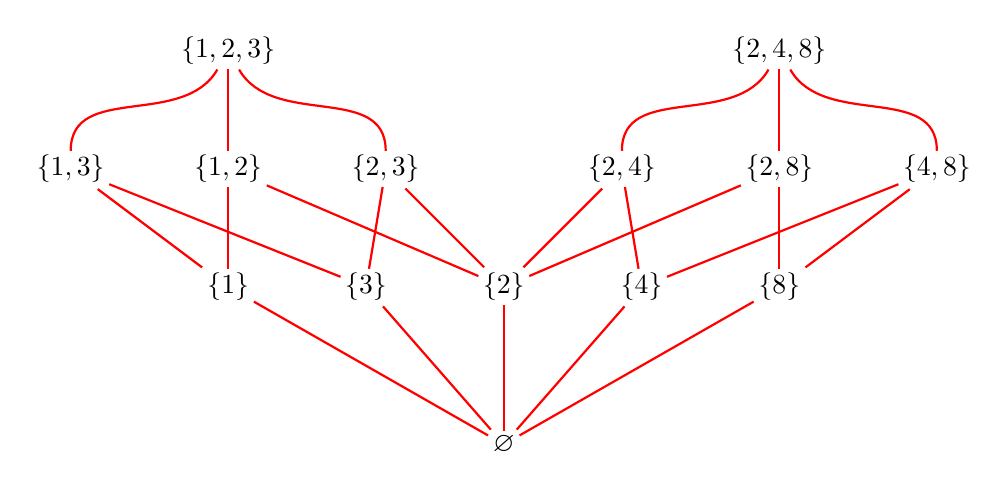
\begin{tikzpicture}
            % First, locate each of the nodes and name them
            \node (topleft) at (0,0) {$\{1,2,3\}$};
            \node (topright) at (7,0) {$\{2,4,8\}$};

            
            \node (set1) at (-2, -1.5)  {$\{1,3\}$};
            \node (set2) at (0, -1.5)  {$\{1,2\}$};
            \node (set3) at (2, -1.5)  {$\{2,3\}$};

            \node (set4) at (5, -1.5)  {$\{2,4\}$};
            \node (set5) at (7, -1.5)  {$\{2,8\}$};
            \node (set6) at (9, -1.5)  {$\{4,8\}$};

            \node (set7) at (0, -3)  {$\{1\}$};
            \node (set8) at (1.75, -3)  {$\{3\}$};
            \node (set9) at (3.5, -3)  {$\{2\}$};
            \node (set10) at (5.25, -3)  {$\{4\}$};
            \node (set11) at (7, -3)  {$\{8\}$};

            \node (emptySet) at (3.5, -5) {$\varnothing$};

            \draw [red,  thick, shorten <=-2pt, shorten >=-2pt, out=-120, in=90] (topleft) to (set1);
            \draw [red,  thick, shorten <=-2pt, shorten >=-2pt, out=-90, in=90] (topleft) to (set2);
            \draw [red,  thick, shorten <=-2pt, shorten >=-2pt, out=-60, in=90] (topleft) to (set3);

            \draw [red,  thick, shorten <=-2pt, shorten >=-2pt, out=-120, in=90] (topright) to (set4);
            \draw [red,  thick, shorten <=-2pt, shorten >=-2pt, out=-90, in=90] (topright) to (set5);
            \draw [red,  thick, shorten <=-2pt, shorten >=-2pt, out=-60, in=90] (topright) to (set6);

            
            % Subsets of {1,3}
            \draw [red,  thick, shorten <=-2pt, shorten >=-2pt] (set1) -- (set8);
            \draw [red,  thick, shorten <=-2pt, shorten >=-2pt] (set1) -- (set7);
            % Subsets of {1,2}
            \draw [red,  thick, shorten <=-2pt, shorten >=-2pt] (set2) -- (set7);
            \draw [red,  thick, shorten <=-2pt, shorten >=-2pt] (set2) -- (set9);
            % Subsets of {2,3}
            \draw [red,  thick, shorten <=-2pt, shorten >=-2pt] (set3) -- (set8);
            \draw [red,  thick, shorten <=-2pt, shorten >=-2pt] (set3) -- (set9);
            % Subsets of {2,4}
            \draw [red,  thick, shorten <=-2pt, shorten >=-2pt] (set4) -- (set9);
            \draw [red,  thick, shorten <=-2pt, shorten >=-2pt] (set4) -- (set10);
            % Subsets of {2,4}
            \draw [red,  thick, shorten <=-2pt, shorten >=-2pt] (set5) -- (set9);
            \draw [red,  thick, shorten <=-2pt, shorten >=-2pt] (set5) -- (set11);
            % Subsets of {4,8}
            \draw [red,  thick, shorten <=-2pt, shorten >=-2pt] (set6) -- (set10);
            \draw [red,  thick, shorten <=-2pt, shorten >=-2pt] (set6) -- (set11);

            % To emptyset
            \draw [red,  thick, shorten <=-2pt, shorten >=-2pt] (set7) -- (emptySet);
            \draw [red,  thick, shorten <=-2pt, shorten >=-2pt] (set8) -- (emptySet);
            \draw [red,  thick, shorten <=-2pt, shorten >=-2pt] (set9) -- (emptySet);
            \draw [red,  thick, shorten <=-2pt, shorten >=-2pt] (set10) -- (emptySet);
            \draw [red,  thick, shorten <=-2pt, shorten >=-2pt] (set11) -- (emptySet);



            
            
        
            % Now draw the lines:
        \end{tikzpicture}
        \end{center}

    \end{homeworkProblem}

    \pagebreak

    \begin{homeworkProblem}

        \question

         A block of cheese is made up of $3\times 3\times 3$ cubes as in the figure below. Is it possible for a mouse to tunnel its way through this block of cheese by (a) starting at a corner, (b) eating its way from cube to adjacent cube, (c) never passing through any cube twice, and, finally, (d) finishing at the center cube? Prove your answer.

        \begin{center}
            \includegraphics[scale = 0.6]{cheese.png}
        \end{center}

        {\em Hint.} This question asks you to find a Hamiltonian path that starts from one of the corner vertices and ends at the center vertex (the only vertex with degree 6). Does such a Hamiltonian path exist?

        \solution 

        There does not exist such a Hamiltonian path. 

        \begin{proof}
            Since the block of cheese is a $3\times 3\times 3$ cube, we know that there must be $27$ vertices (with coordinates $(x,y,z))$. 
        
            WLOG, suppose our corner vertex where we start is $(0,0,0)$, Let the coordinate of the center vertex be $(1,1,1)$. Consider the sum of coordinates (parity $= x+y+z$) for the corner vertex and center vertex: The corner vertex has a even parity and the center vertex has an odd parity. 
        
            Everytime we traverse along an edge to a vertex, only \textit{one} of our coordinates gets shifted along by one (either $x$, $y$ or $z$) which means the parity changes from even to odd to even to odd and so forth. 
            
            One can observe that a Hamiltonian path that travels along $27$ vertices must have $26$ edges. Therefore since $26$ is even we will have that the parity of the final vertex will be the same as the starting vertex (even). 

            However we know that the parity of $(1,1,1)$ the center vertex is odd hence there is no Hamiltonian path that starts from one of the corner vertices and ends at a center vertex.
        \end{proof}

        

    \end{homeworkProblem}





    








    \end{document}